%% Manuscript prepared with the Elsevier elsarticle class (numbered references), intended for
%% Biomedical Signal Processing and Control. Tables are \input from tables/, generated together with
%% the figures by make_figures.py from the evaluation records; do not edit those files by hand.
\documentclass[preprint,12pt]{elsarticle}

\usepackage[T1]{fontenc}
\usepackage[utf8]{inputenc}
\usepackage{amsmath,amssymb}
\usepackage{graphicx}
\usepackage{booktabs}
\usepackage{array}
\usepackage{multirow}
\usepackage{rotating}
\usepackage{lineno}
\usepackage[hidelinks]{hyperref}

% Table bodies are generated files; the TeX primitive input keeps \bottomrule valid after them.
\makeatletter
\newcommand{\tablebody}[1]{\@@input #1 }
\makeatother

\newcommand{\Sarm}{S_{\mathrm{arm}}}
\newcommand{\Sreal}{S_{\mathrm{real}}}
\newcommand{\vdac}{V_{\mathrm{DAC}}}
\newcommand{\sibi}{\sigma_{\tau}}

\journal{Biomedical Signal Processing and Control}

\begin{document}

\begin{frontmatter}

\title{Rate-controllable photoplethysmogram synthesis with a constructed rhythm: a GAN and a rectified-flow model under pre-specified evaluation}

%% TODO(authors): replace with full names as they should appear, add ORCID iDs and the corresponding
%% author's e-mail. The project README lists the authors as HuyNN and VyPT.
\author[iuh]{[First author]\corref{cor1}}
\ead{[corresponding author e-mail]}
\author[iuh]{[Second author]}
\cortext[cor1]{Corresponding author.}
\affiliation[iuh]{organization={Faculty of Electronic Technology, Industrial University of Ho Chi Minh City},
            city={Ho Chi Minh City},
            country={Vietnam}}

\begin{abstract}
Synthetic photoplethysmograms (PPG) are used to test pulse-rate and rhythm algorithms, but parametric pulses are easy to tell apart from recorded PPG, and learned generators rarely follow a commanded rate. We present two conditional generators that construct the beat sequence from the commanded rate and irregularity and learn only pulse morphology and texture: PhysioMix, a generative adversarial network (0.16\,M parameters), and PhysioFlow, a rectified-flow U-Net (6.9\,M parameters). Both were trained on six public datasets with subject-disjoint splits and selected on validation data under decision rules written before training. Their mean absolute rate error was below 1\,bpm from 40 to 180\,bpm. On subjects never used for training, a subject-grouped classifier two-sample test rated PhysioFlow 50--91\% indistinguishable from real windows on four finger and intensive-care datasets, against 7--45\% for PhysioMix and 0\% for a parametric Gaussian pulse; a frozen PPG foundation model ranked the generators similarly (Spearman $\rho=0.88$). Three published beat detectors, however, estimated the rate within 5\,bpm on 88--100\% of generated strips, against 19--26\% of real wrist-exercise windows and 75--77\% of everyday wrist windows: like the Gaussian pulse, the generators did not reproduce the difficulty of motion-corrupted PPG. Neither model transferred to everyday wrist PPG from an unseen device (below 1\% indistinguishable); retraining with that device's data raised the flow model to 33\%, short of the pre-specified margin. Both generators run in a Raspberry Pi 4 bench simulator whose optical path is not yet validated.
\end{abstract}

\begin{keyword}
Photoplethysmography \sep Synthetic physiological signals \sep Generative adversarial network \sep Rectified flow \sep Pre-specified evaluation \sep Beat detection
\end{keyword}

\end{frontmatter}

% Line numbers for review start after the title page: on it, lineno pushes the
% corresponding-author footnote into the preprint footer.
\linenumbers

%% ================================================================================================
\section{Introduction}
\label{sec:intro}

Photoplethysmography (PPG) measures changes in tissue blood volume optically. It is the sensing principle behind pulse oximeters, smartwatches and many bedside and ambulatory monitors \cite{allen2007ppg,charlton2022wearable}. Algorithms that run on the PPG estimate pulse rate, detect atrial fibrillation, extract respiratory rate and grade signal quality \cite{charlton2018breathing,park2022review,elgendi2012analysis}, and denoising methods are being developed for the motion-corrupted signals of wearables \cite{bradley2024envelope,jain2024ssl}. Before such algorithms, and the devices that run them, can be trusted, they have to be tested on signals whose properties are known.

Two kinds of test signal are in use. Recorded databases contain real physiology, and a beat detector can be scored against them \cite{charlton2022beats}, but they cannot be varied: rate, rhythm and recording conditions are fixed by the recording. Synthetic signals reverse the trade-off. Commercial functional testers modulate light with a pulse whose rate, amplitude and timing features are set by the operator; the WhaleTeq AECG100, for example, covers 10--300\,bpm with PPG, sine, triangle and square waveforms \cite{whaleteq2025manual}. Such testers show that a device responds, but they do not establish SpO$_2$ accuracy, which is assessed in controlled studies on human subjects \cite{iso80601}. Academic simulators follow the same pattern, from LED rigs that replay database PPG \cite{pittella2024optical} or interval series of ventricular tachycardia \cite{solosenko2024vt} to software frameworks that combine parametric pulses with rhythm and noise models \cite{karhinoja2026flexible}.

The waveform is the weak point of these systems. Parametric models built from sums of Gaussians \cite{mcsharry2003ecg,tang2020gaussian}, stochastic pulse models \cite{martin2013stochastic}, rhythm models of atrial fibrillation \cite{solosenko2017af,solosenko2022physionet} and haemodynamic pulse-wave databases \cite{charlton2019pwdb} give exact control, but their pulses repeat more regularly than real ones \cite{mejia2022synthesis}. In our evaluation, a small convolutional classifier separated a Gaussian pulse from real windows of unseen subjects in all six datasets. Deep generative models fill part of this gap. Generative adversarial networks (GANs) \cite{goodfellow2014gan} have produced PPG for data augmentation \cite{kiyasseh2020pleth,ding2023lsmgan}, guided diffusion has generated PPG from a few examples \cite{kang2024bgdiff}, and diffusion and flow-matching models now generate electrocardiograms, translate between PPG and ECG or produce several cardiovascular signals with one network \cite{alcaraz2023sssd,bondar2025flowecg,sarkar2021cardiogan,shome2024rddm,chen2026unicardio}. These models were not built to follow an operator's rate command, and their realism is often judged on a few examples, with a single distance or on test data that were seen during development \cite{brophy2023gan,theis2016note}.

A generator that is to serve as a test signal has four requirements. The rate and rhythm must follow the command exactly, including outside the range that dominates the training data. The waveform should be realistic in the recording context the user selects, such as a fingertip at rest, a patient in intensive care or a wrist during exercise. Inference has to fit a small computer that also drives a test rig in real time. Finally, users need to know where the model is realistic, and whether algorithms behave on its output as they do on real data; this requires evaluation on unseen subjects with metrics that a generator cannot easily satisfy by accident. The last requirement also concerns model selection. When the same validation subjects are reused over many development rounds, validation scores become optimistic, and gains reported on them may not survive a fresh test \cite{varoquaux2022failures,saeb2017usecase}. Fixing the analysis before the data are seen is the standard remedy in other fields \cite{nosek2018prereg}, and we apply it here to the development of signal generators.

This paper describes how we addressed these requirements and where we fell short. Its contributions are:
\begin{itemize}
\item two conditional generators, PhysioMix (a GAN) and PhysioFlow (a rectified-flow model), that construct the beat sequence from the rate and irregularity commands and learn only the waveform around it (Section~\ref{sec:generators});
\item a selection protocol in which every decision rule was written and committed before training and applied to validation data only, complemented by realism measurements on unseen subjects: precision and recall in a descriptor space, a subject-grouped classifier two-sample test with subject-bootstrap intervals, a frozen PPG foundation model, recording-context classification, memorisation screening and a fresh test on everyday wrist PPG (Section~\ref{sec:protocol});
\item a utility test in which three published beat detectors are run on real recordings with an independent reference rate and on generated strips at the same rates (Section~\ref{sec:detector-protocol});
\item results that include negative findings: exact rate control in both models, a clear realism advantage of rectified flow on finger and intensive-care data, strips that are easier for beat detectors than the real recordings, the failure of both models on everyday wrist PPG from an unseen device, and two cases in which the pre-specified rules kept the deployed model unchanged (Section~\ref{sec:results}).
\end{itemize}
The generators were built for a Raspberry Pi 4 bench simulator that drives red and infrared LEDs; Section~\ref{sec:platform} summarises it and \ref{app:hardware} gives the hardware and its timing measurements. The optical path of that simulator has not been validated, and this paper makes no claim about it.

%% ================================================================================================
\section{Target platform and parametric baseline}
\label{sec:platform}

\begin{figure}[tbp]
\centering
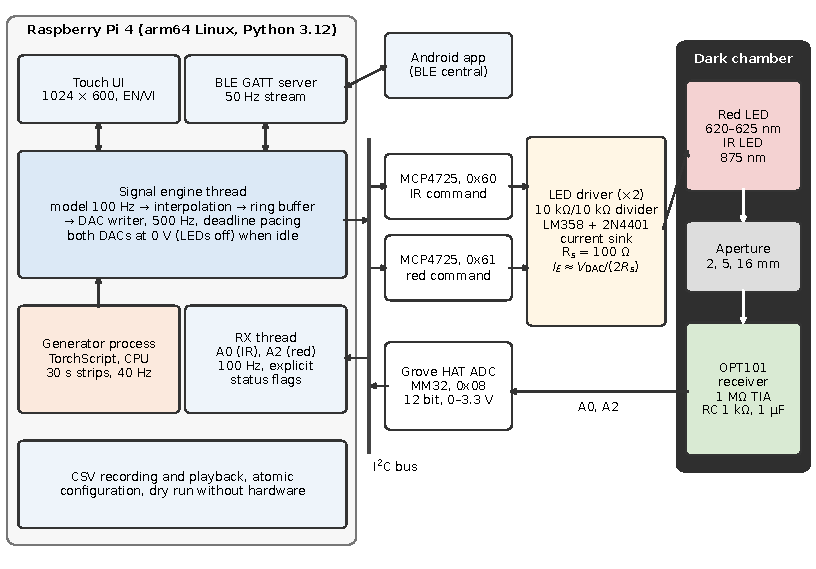
\includegraphics[width=\textwidth]{figures/fig1_system.pdf}
\caption{Architecture of the bench simulator for which the generators were built. Software threads and the generator process run on the Raspberry Pi; the two converters and the receiver ADC share one I$^2$C bus. The hardware is described in \ref{app:hardware}; its optical path has not been validated. Diagram drawn with Matplotlib from code written with the help of Claude (Anthropic).}
\label{fig:system}
\end{figure}

\subsection{Simulator context}
\label{sec:context}

The simulator (Fig.~\ref{fig:system}) runs on a Raspberry Pi 4 Model B and writes two MCP4725 12-bit converters \cite{mcp4725ds}, one per LED channel, from a single signal-engine thread at 500\,Hz by default. The application is written in Python 3.12. Learned generators never run on the engine or interface threads: the interface starts a worker process that loads a TorchScript generator, produces one 30\,s strip at 40\,Hz and returns it. A generated strip $x(t)\in[0,1]$ is mapped to commanded voltages
\begin{equation}
v_{\mathrm{IR}}(t) = V_{\mathrm{DC}} + A_{\mathrm{IR}}\,x(t), \qquad v_{\mathrm{red}}(t) = V_{\mathrm{DC}} + 0.48\,A_{\mathrm{IR}}\,x(t),
\label{eq:mapping}
\end{equation}
with $V_{\mathrm{DC}}=1.5$\,V and $A_{\mathrm{IR}}=45$\,mV by default, both adjustable. The fixed red-to-infrared ratio is a nominal mapping, not a learned optical relation. The strip is interpolated linearly to 100\,Hz and then to the converter rate; interpolation adds no bandwidth. A dry-run mode replaces all hardware access, so the complete application, its automated test suite of more than 800 tests and every generator measurement in this paper run on a laptop.

\subsection{Parametric pulse}
\label{sec:parametric}

The conventional mode reproduces the PPG controls of commercial testers \cite{whaleteq2025manual} and provides the Gaussian baseline of the evaluation. Like other parametric PPG models, it builds each cycle from Gaussian components that stand for the forward (systolic) and reflected (diastolic) waves \cite{tang2020gaussian,mejia2022synthesis}. With the cycle phase $\vartheta\in[0,1)$ and the unit-height Gaussian $g$,
\begin{equation}
\begin{aligned}
g(\vartheta;\mu,\sigma) &= \exp\!\bigl(-(\vartheta-\mu)^2/2\sigma^2\bigr),\\
\tilde{P}(\vartheta) &= E(\vartheta)\,\bigl[g(\vartheta;\mu_{\mathrm S},\sigma_{\mathrm S}) + \alpha_{\mathrm D}\,g(\vartheta;\mu_{\mathrm D},\sigma_{\mathrm D})\bigr]\,\bigl[1-\eta\,g(\vartheta;\mu_{\mathrm N},\sigma_{\mathrm N})\bigr],\\
P(\vartheta) &= \tilde{P}(\vartheta)\big/\max_{\vartheta'}\tilde{P}(\vartheta'),
\end{aligned}
\label{eq:gauss}
\end{equation}
where $\alpha_{\mathrm D}=0.4$ is the diastolic weight and $\eta=0.25$ the depth of a local notch attenuation. The default centres are $\mu_{\mathrm S}=0.15$, $\mu_{\mathrm N}=0.30$ and $\mu_{\mathrm D}=0.40$ and the widths $\sigma_{\mathrm S}=0.055$, $\sigma_{\mathrm N}=0.02$ and $\sigma_{\mathrm D}=0.10$, in fractions of a cycle; they are specified at 60\,bpm and scale with the cycle length. The taper $E$ is a smoothstep over the first and last 5\% of the cycle, which makes the pulse and its slope continuous from one cycle to the next. Two positive Gaussians alone already leave a valley between the systolic and diastolic peaks \cite{tang2020gaussian}; the multiplicative notch term deepens it without ever making the pulse negative. It is an engineering choice, not a model of valve closure, and the default timings form a simulator template rather than values fitted to a population.

Each channel has its own DC level $V_{\mathrm{DC}}$ and AC amplitude $A$, and the perfusion index is $\mathrm{PI}=100\,A_{\mathrm{IR}}/V_{\mathrm{DC,IR}}$. A target saturation sets the ratio of ratios through the empirical linear calibration used by pulse oximeters and by the commercial tester \cite{webster1997pulse,whaleteq2025manual},
\begin{equation}
\begin{aligned}
\mathrm{SpO_2} &= k_1 - k_2\,R, \qquad R=\frac{A_{\mathrm{red}}/V_{\mathrm{DC,red}}}{A_{\mathrm{IR}}/V_{\mathrm{DC,IR}}},\\
A_{\mathrm{red}} &= \frac{k_1-\mathrm{SpO_2}}{k_2}\,A_{\mathrm{IR}}\,\frac{V_{\mathrm{DC,red}}}{V_{\mathrm{DC,IR}}},
\end{aligned}
\label{eq:ratio}
\end{equation}
with $k_1=110$ and $k_2=25$ by default. Respiration modulates baseline, amplitude and beat timing at 1--150 breaths/min with an adjustable inspiration-to-expiration ratio and optional apnoea \cite{charlton2018breathing}, and the heart rate spans 10--300\,bpm. Because $R$ is set rather than measured, this mode commands an optical ratio; it does not turn the simulator into an SpO$_2$ calibrator. For the evaluation, the pulse of Eq.~\eqref{eq:gauss} is rendered at the commanded rate, without respiration or noise, and passed through the data view of Section~\ref{sec:view}.

%% ================================================================================================
\section{Rhythm-scaffolded generators}
\label{sec:generators}

\begin{figure}[tbp]
\centering
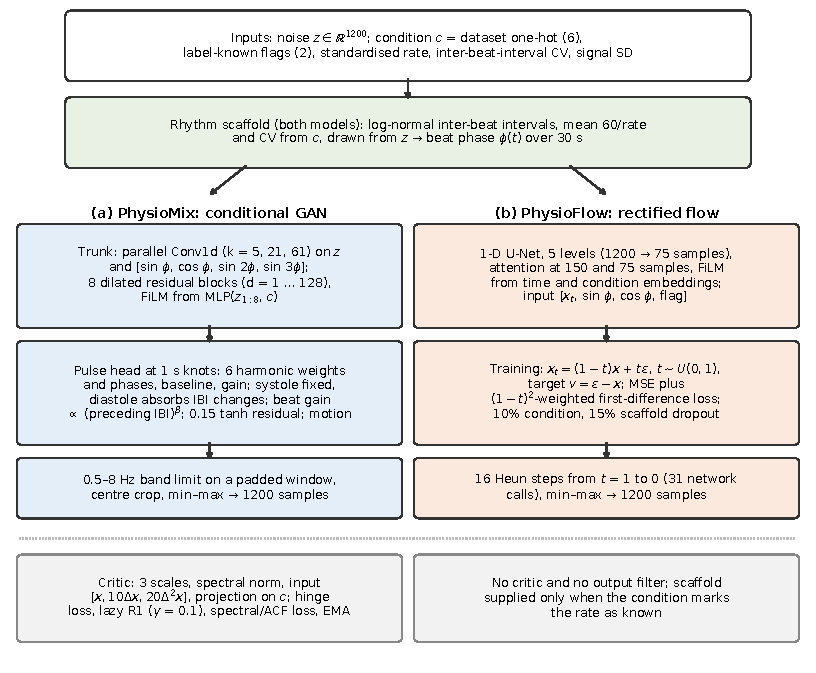
\includegraphics[width=\textwidth]{figures/fig3_generators.pdf}
\caption{The two generators share the inputs and the rhythm scaffold, which fixes the beat times from the rate and irregularity commands. (a) PhysioMix shapes each beat with a convolutional trunk and harmonic pulse head and is trained against a multi-scale critic. (b) PhysioFlow learns a velocity field with a one-dimensional U-Net and generates by integrating it from noise. Symbols as in Eqs.~\eqref{eq:ibi}--\eqref{eq:flow}. Diagram drawn with Matplotlib from code written with the help of Claude (Anthropic).}
\label{fig:generators}
\end{figure}

\subsection{Data view and condition vector}
\label{sec:view}

All learned models work on the same view of the data. The mean of each record is removed, the record is resampled to 40\,Hz (polyphase resampling with linear edge padding) and filtered by a fourth-order Butterworth band-pass from 0.5 to 8\,Hz applied forwards and backwards, which gives a zero-phase response. The filtered record is cut into non-overlapping 30\,s windows (1200 samples), and each window $x$ is scaled to $[0,1]$ by its own minimum and maximum. Windows whose raw signal was flat or spent more than 5\% of its samples at its minimum or maximum (clipping) were discarded. The view keeps the pulse and its harmonics up to 8\,Hz but removes the slow respiratory baseline and the absolute amplitude, so the generators learn normalised shape and timing only.

The condition vector $c\in\mathbb{R}^{11}$ contains a one-hot code for the six training datasets, two flags that state whether the window's rate and irregularity labels are known, and three values standardised with training statistics: pulse rate, coefficient of variation (CV) of the inter-beat intervals (IBIs) and the standard deviation of the window. (The models retrained in Section~\ref{sec:wrist-protocol} with a seventh dataset code have $c\in\mathbb{R}^{12}$.) Rate labels come from the agreement of spectral, autocorrelation and beat-interval estimates; where an ECG is available, the ECG rate is used when the PPG estimate agrees with it, and the label is masked otherwise. On the finger dataset described below, the median absolute difference between the PPG and ECG rates was 0.47\,bpm. Wrist PPG during exercise is dominated by motion: its PPG rate differed from the ECG rate by a median of 52\,bpm, and 86\% of its rate labels were masked. For a masked label, the flag is set to zero and the value is replaced by one drawn at random from the known labels of the same dataset, so that the standardised entry carries no information that the flag does not already give. In the application, the user's command sets both flags to one.

\subsection{Rhythm scaffold}
\label{sec:scaffold}

Both generators construct the beat sequence instead of learning it. Given a rate command $r$ (bpm), with $f=r/60$, and an irregularity command $\sibi\in[0,0.35]$, the IBIs are drawn as
\begin{equation}
\tau_k = \frac{\exp\!\left(\sibi u_k - \sibi^2/2\right)}{f}, \qquad u_k\sim\mathcal{N}(0,1),
\label{eq:ibi}
\end{equation}
so that $\mathbb{E}[\tau_k]=1/f$ for any $\sibi$. The intervals are log-normal with log-scale standard deviation $\sibi$; their CV, $\sqrt{\exp(\sibi^2)-1}$, equals $\sibi$ to within 3.5\% over the allowed range (0.202 at $\sibi=0.20$, 0.361 at 0.35), so $\sibi$ is used as the IBI CV command. The $u_k$ are read from the generator's noise vector, and a random fraction of the first interval sets the phase at the start of the window. Cumulative sums give beat onsets (PhysioMix) or systolic peak times (PhysioFlow), and the beat phase
\begin{equation}
\phi(t)=2\pi\,[\,j(t)+\delta(t)\,]
\label{eq:phase}
\end{equation}
combines the index $j(t)$ of the current beat with the elapsed fraction $\delta(t)\in[0,1)$ of its interval. Because the networks see only $\phi(t)$, the rate cannot drift away from the command, and commands outside the label range of the training data remain valid. The log-normal law describes the dispersion of the intervals but not their sequential structure, so it is not a validated model of atrial fibrillation.

\subsection{PhysioMix: a conditional GAN}
\label{sec:physiomix}

PhysioMix (Fig.~\ref{fig:generators}a) turns the scaffold into a waveform with 162{,}216 parameters. A trunk of three parallel one-dimensional convolutions (kernels of 5, 21 and 61 samples, 16 channels each) reads the noise $z\in\mathbb{R}^{1200}$ and four carriers ($\sin\phi$, $\cos\phi$, $\sin2\phi$ and $\sin3\phi$) and feeds eight residual blocks with 48 channels and dilations from 1 to 128, in the manner of temporal convolutional networks \cite{bai2018tcn}. Each block is modulated by feature-wise linear modulation (FiLM) \cite{perez2018film} from a style vector that a small perceptron computes from $c$ and the first eight noise values. A head averages the trunk over 1\,s and predicts, at each 1\,s knot, six harmonic weights $a_h\ge0$ normalised to $\sum_h a_h=1$, their phases $\psi_h$, a baseline $b$ and a gain $G\in[e^{-1/2},e^{1/2}]$; the knots are interpolated linearly back to 40\,Hz. Before normalisation the output is
\begin{equation}
y(t) = G(t)\sum_{h=1}^{6} a_h(t)\,\sin\!\bigl(h\,\phi(t)+\psi_h(t)\bigr) + b(t) + 0.15\tanh\zeta(t) + m(t),
\label{eq:physiomix}
\end{equation}
where $\zeta(t)$ is a free residual from the trunk; its bound keeps it from overriding the rhythm. Three further details make the beats more physiological. Systole keeps a fixed duration of $0.35/f$, and diastole absorbs the interval changes: $\delta(t)$ advances linearly to 0.35 over the systolic part of each beat and then to 1 over the rest of the interval, so the peak-to-peak intervals keep the commanded dispersion. Each pulse is scaled by $(\tau_{k-1}f)^{\beta}$, with $\beta\in[0,1]$ predicted from the style vector, which mimics the dependence of pulse amplitude on the preceding filling time; the new gain ramps in over the first 20\% of the beat. A periodic motion term $m(t)$, with a cadence of 0.5--3.5\,Hz that is constant within a window, three harmonics and an amplitude of at most 1.5, all predicted from the style vector, represents wrist motion as a waveform; it is not driven by an accelerometer. The signal is generated with 240 extra samples (6\,s) on each side, band-limited with the magnitude response of the data-view filter, cropped to the central 30\,s and min--max normalised to give $x(t)$.

The critic examines a window $x$ together with its scaled differences $10\Delta x$ and $20\Delta^2x$ at three time scales, with spectral normalisation \cite{miyato2018spectral} and a projection term on $c$ \cite{miyato2018projection}. We trained with the hinge loss \cite{lim2017geometric}, $\mathcal{L}_D=\mathbb{E}[\max(0,1-D(x_{\mathrm{real}},c))]+\tfrac12\mathbb{E}[\max(0,1+D(x_{\mathrm{gen}},c))]+\tfrac12\mathcal{L}_{\mathrm{mis}}$, where the mismatch term $\mathcal{L}_{\mathrm{mis}}$ treats real windows paired with a wrong condition (another dataset, or a known rate more than 10\,bpm away) as negatives. Lazy R1 regularisation \cite{mescheder2018convergence,karras2020stylegan2} was applied every 16 steps with weight 0.1, and the critic gradient was clipped at norm 10 (160 on R1 steps, to account for the 16-fold scaling of lazy R1). The generator minimises $-\mathbb{E}[D(x_{\mathrm{gen}},c)]+\tfrac12\mathcal{L}_{\mathrm{dist}}+\tfrac12\mathcal{L}_{\mathrm{dist}}^{\mathrm{dataset}}$, where $\mathcal{L}_{\mathrm{dist}}$ compares the distributions of generated and real batches without pairing windows: it sorts, across the batch, the normalised log power spectra (Hann-windowed blocks of 4, 10 and 20\,s with 50\% overlap) and the autocorrelation functions (lags up to 5\,s), and takes the smooth-L1 distance between the sorted spectra and the squared distance between the sorted autocorrelations; and $\mathcal{L}_{\mathrm{dist}}^{\mathrm{dataset}}$ is the same loss computed within each dataset of the batch. Optimisation used Adam \cite{kingma2015adam} with momentum parameters $(0, 0.99)$, a learning rate of $10^{-4}$ decayed by a cosine schedule to $10^{-5}$, batches of 32, 20{,}000 updates, generator gradient clipping at norm 10 and an exponential moving average of the generator weights with decay 0.995 \cite{yazici2019ema}.

\subsection{PhysioFlow: conditional rectified flow}
\label{sec:physioflow}

PhysioFlow (Fig.~\ref{fig:generators}b) replaces the adversarial game by rectified flow \cite{liu2023rectified}, a form of flow matching \cite{lipman2023flow}. Let $x_0$ be a real window standardised to zero mean and unit variance, $\varepsilon\sim\mathcal{N}(0,I)$, and let the flow time $s\sim\mathcal{U}(0,1)$ (distinct from the signal time $t$). A network $v_\theta$ is trained on the straight path $x_s=(1-s)\,x_0+s\,\varepsilon$ to predict the velocity $\varepsilon-x_0$:
\begin{equation}
\begin{aligned}
\mathcal{L} &= \mathbb{E}\,\bigl\|v_\theta(x_s,s,\Phi,c)-(\varepsilon-x_0)\bigr\|^2 + \omega\,\mathbb{E}\,\Bigl[(1-s)^2\,\bigl\|10\,(\Delta\hat{x}_0-\Delta x_0)\bigr\|^2\Bigr],\\
\hat{x}_0 &= x_s - s\,v_\theta(x_s,s,\Phi,c),
\end{aligned}
\label{eq:flow}
\end{equation}
where $\|\cdot\|^2$ denotes the mean over samples, $\Phi=[\sin\phi,\cos\phi,\text{flag}]$ are the three scaffold channels, and the second term ($\omega=1$) penalises errors in the first difference of the implied clean signal, weighted towards low noise levels. The network is a one-dimensional U-Net \cite{ronneberger2015unet} with five resolutions (1200 down to 75 samples), 32, 64, 128, 160 and 160 channels, two residual blocks per level, self-attention at 150 and 75 samples and FiLM modulation from flow-time and condition embeddings; it has 6{,}923{,}137 parameters. Its input concatenates $x_s$ with $\Phi$. The scaffold is supplied only when the condition marks the rate as known, as in training, where windows with masked labels were learned without it; a further 15\% of training windows drop the scaffold and 10\% drop the condition, which would allow classifier-free guidance \cite{ho2022cfg}. Sampling integrates $\mathrm{d}x/\mathrm{d}s=v_\theta$ from $s=1$ to 0 with 16 steps of Heun's method \cite{karras2022edm} (31 network evaluations, the last step being an Euler step) without guidance, and min--max normalises the result. PhysioFlow has no critic and no output filter. Training used AdamW with momentum parameters $(0.9, 0.99)$, weight decay 0.01, a learning rate of $3\times10^{-4}$ with a cosine schedule, batches of 128, 20{,}000 updates, gradient clipping at norm 1 and an exponential moving average of the weights with decay $\min\bigl(0.999,(1+n)/(10+n)\bigr)$ at update $n$.

\subsection{Baselines and variants}
\label{sec:baselines}

Three references accompany the two generators. The \emph{Gaussian} baseline is the parametric pulse of Eq.~\eqref{eq:gauss}. \emph{LSM-GAN} is the generator previously deployed in the simulator, a log-spectral-matching GAN \cite{ding2023lsmgan} with 117{,}940 parameters that maps noise to a 30\,s sequence; it was trained on BIDMC in a 0.9--5\,Hz band and has no condition input. \emph{Real (other subjects)} scores real windows of training subjects in place of a generator, which shows the level that a different real person reaches under each metric. One variant appears in the development history: \emph{PhysioFlow-SB} adds to Eq.~\eqref{eq:flow} a loss on the log power spectrum in the stop bands of the data view (weight 0.1). The models retrained with everyday wrist data, PhysioMix-G, -D and PhysioFlow-G, -D, -E, are described in Section~\ref{sec:wrist-protocol}; the retrained flow models all use the PhysioFlow-SB recipe. Fig.~\ref{fig:waveforms} shows strips of the three generators next to real test windows, and Table~\ref{tab:generators} gives their size and speed.

\begin{figure}[tbp]
\centering
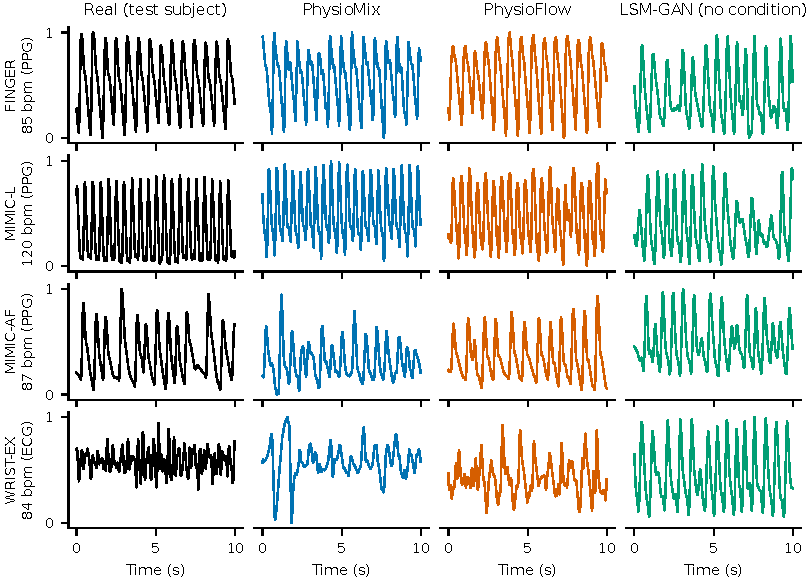
\includegraphics[width=\textwidth]{figures/fig4_waveforms.pdf}
\caption{Ten-second excerpts of 30\,s strips. The left column shows a randomly drawn test window of each dataset; PhysioMix and PhysioFlow were prompted with that window's dataset, its rate (PPG-derived, or ECG-derived for WRIST-EX) and the dataset's default irregularity, with the same noise seed for every row. LSM-GAN takes no condition and was given a different seed per row.}
\label{fig:waveforms}
\end{figure}

\begin{table}[tbp]
\centering
\caption{Generator footprint. Latency is the median of seven generations of one 30\,s strip after a warm-up, on one core of an AMD Ryzen~7 8840HS laptop with PyTorch 2.10.0 \cite{paszke2019pytorch}.}
\label{tab:generators}
\small
\begin{tabular}{lrlr}
\toprule
Generator & Parameters & Type & Latency (ms) \\
\midrule
\tablebody{tables/generators.tex}
\bottomrule
\end{tabular}
\end{table}

%% ================================================================================================
\section{Evaluation protocol}
\label{sec:protocol}

\subsection{Datasets and splits}
\label{sec:data}

Table~\ref{tab:datasets} lists the training data. The six datasets come from four public sources \cite{li2026data,li2026mendeley,charlton2022beats,charlton2025mimicperform,pimentel2017rr,goldberger2000physionet,jarchi2017wrist}; all recordings are de-identified, and no new data were collected from human participants for this study. They cover healthy adults at rest and after exercise (FINGER), critically ill adults (BIDMC and MIMIC-L, the latter derived from MIMIC-III \cite{johnson2016mimic}) including patients in atrial fibrillation (MIMIC-AF) and in sinus rhythm (MIMIC-nonAF), and healthy adults exercising with a wrist sensor (WRIST-EX). Each dataset was split by subject with a fixed seed, so no subject contributes to more than one split \cite{saeb2017usecase}. For MIMIC-L, subjects are waveform record groups, because unique patient identities could not be verified; known aliases between the AF records and the larger set were joined before splitting, and possible overlap between BIDMC and MIMIC-derived records was handled by excluding matching record identifiers. Windows whose first or last 2\,s exceeded the middle 1--99\% range of the window by more than 50\% were removed from every split. The FINGER infrared channel is inverted by the recording device and was negated; 433 of 444 records showed a consistent pulse delay after the ECG R peak, and the remaining 11 were excluded. The prepared data pack carries a SHA-256 digest that every training and evaluation run checked. Two further sources were kept out of training altogether: GalaxyPPG (Section~\ref{sec:wrist-protocol}) and CapnoBase \cite{karlen2013capnobase}, which was reserved for external evaluation and entered no decision.

\begin{sidewaystable}
\centering
\caption{Training datasets and subject-disjoint splits. Cells give subjects / 30\,s windows. MIMIC-L subjects are waveform record groups.}
\label{tab:datasets}
\footnotesize
\setlength{\tabcolsep}{4pt}
\begin{tabular}{ll>{\raggedright\arraybackslash}p{5.0cm}rrrr}
\toprule
Dataset & Source & Recording & $f_s$ (Hz) & Train & Validation & Test \\
\midrule
\tablebody{tables/datasets.tex}
\bottomrule
\end{tabular}
\end{sidewaystable}

\subsection{Locked validation criterion}
\label{sec:criterion}

Checkpoint and model selection used one criterion. It was frozen before the third development round, identified by its SHA-256 digest and not changed afterwards. For each validation pool $d$, generated windows are prompted with condition vectors drawn from the training windows of that dataset and compared with up to 256 subject-balanced validation windows:
\begin{equation}
\begin{aligned}
Q_d ={}& \mathrm{MMD}^2_{\mathrm{ACF}} + \mathrm{MMD}^2_{\mathrm{PSD}} + \mathrm{MMD}^2_{\mathrm{morph}}\\
&+ 0.5\,(1-\mathrm{recall}_d) + 0.25\,(1-\mathrm{precision}_d).
\end{aligned}
\label{eq:q}
\end{equation}
The three squared maximum mean discrepancies \cite{gretton2012mmd} use Gaussian kernels with median-heuristic bandwidths on autocorrelation functions, log power spectra and nine morphology descriptors: rate, IBI CV, pulse width at half height, rise time, standard deviation, skewness, mean absolute slope, mean absolute curvature and the fraction of power above 5\,Hz. Precision and recall are $k$-nearest-neighbour manifold estimates \cite{kynkaanniemi2019pr} in the same descriptor space, standardised with training statistics. With $\Psi$ the standardised descriptors, $\{x_i\}_{i=1}^{N}$ the real and $\{\tilde{x}_j\}_{j=1}^{M}$ the generated windows, and $\rho_5(\cdot)$ the distance from a window to its fifth-nearest neighbour within its own set,
\begin{equation}
\begin{aligned}
\mathrm{precision}&=\frac1M\sum_{j=1}^{M}\mathbb{1}\!\left[\exists i:\ \|\Psi(\tilde{x}_j)-\Psi(x_i)\|\le\rho_5(x_i)\right],\\
\mathrm{recall}&=\frac1N\sum_{i=1}^{N}\mathbb{1}\!\left[\exists j:\ \|\Psi(x_i)-\Psi(\tilde{x}_j)\|\le\rho_5(\tilde{x}_j)\right].
\end{aligned}
\label{eq:pr}
\end{equation}
Precision is the share of generated windows that look like some real window (often called fidelity), and recall is the share of real windows that the generator covers. The pools are weighted 0.35 (FINGER), 0.25 (MIMIC-L), 0.15 (BIDMC), 0.15 (MIMIC-AF and MIMIC-nonAF together) and 0.10 (WRIST-EX), and
\begin{equation}
\Sreal = \sum_d w_d\,Q_d + 0.25\,\lvert\ln\nu\rvert,
\label{eq:sreal}
\end{equation}
where $\nu$ is the ratio of the median pairwise distance among generated windows to that among domain-matched real training windows; the term penalises collapsed or over-dispersed output. Controllability is scored on a grid of rates from 40 to 180\,bpm in steps of 10\,bpm, with eight samples per point and dataset and a peak-based rate estimator that is independent of the generator:
\begin{equation}
\begin{aligned}
C ={}& 0.5\min\!\left(\frac{\mathrm{MAE_{in}}}{10},2\right) + 0.25\min\!\left(\frac{\mathrm{MAE_{ext}}}{10},2\right)\\
&+ 0.25\,(1-\rho_S) + 0.25\,(1-\mathrm{AUC_{irr}}).
\end{aligned}
\label{eq:c}
\end{equation}
Here $\mathrm{MAE_{in}}$ and $\mathrm{MAE_{ext}}$ are the mean absolute rate errors in bpm inside and outside 60--140\,bpm (an undetected rate counts as 20\,bpm), $\rho_S$ is the Spearman correlation between commanded and median measured rate, averaged over datasets, and $\mathrm{AUC_{irr}}$ is the area under the receiver operating characteristic curve for separating irregular ($\sibi=0.20$) from regular ($\sibi=0.02$) prompts at the rates inside 60--140\,bpm by the root mean square of successive interval differences \cite{taskforce1996hrv}. The score of a trained model adds a classifier two-sample test (C2ST) \cite{lopezpaz2017c2st}:
\begin{equation}
\Sarm = \Sreal + 0.5\,C + 0.5\max\left(0,\mathrm{AUC_{C2ST}}-0.5\right),
\label{eq:sarm}
\end{equation}
where $\mathrm{AUC_{C2ST}}$ is the validation AUC of a small convolutional probe (three strided convolutions with 16, 32 and 32 channels and about 11\,k parameters) that sees the window and its first two differences. Lower values are better for $Q_d$, $\Sreal$, $C$ and $\Sarm$. A model also had to pass gates: finite output, no flat windows, no non-finite losses, critic gradient clipping in at most 1\% of updates, $\nu\in[0.75,1.25]$, numerical agreement between the exported TorchScript and the checkpoint, and single-thread latency below 50\,ms (GAN) or 5\,s (flow) per 30\,s window.

\subsection{Pre-specified decision rules}
\label{sec:rules}

Each development round followed the same procedure. A rule naming the candidate, the incumbent and the conditions for replacing the incumbent was written to a file, hashed with SHA-256 and committed to the project's version control before training. Candidates were trained with three seeds (42, 123 and 2026) on two NVIDIA T4 GPUs, and checkpoints were chosen every 500 (GAN) or 2000 (flow) updates on validation $\Sreal+0.5C$ computed with the averaged weights. The general rule replaced the incumbent only if every seed passed the gates, the mean $\Sarm$ was lower by more than the pooled seed standard deviation, and the mean $\Sreal$ was not worse by more than 0.05. Round 9 targeted the wrist dataset instead: it required a wrist $Q$ better than the incumbent's by more than the pooled standard deviation while $\Sarm$ stayed within one pooled standard deviation of the incumbent. Because round 9 had been accepted for its wrist gain, later rules added a wrist guard: the mean wrist $Q$ could not be worse than the incumbent's by more than the pooled standard deviation. The deployed seed was the candidate's lowest-$\Sarm$ seed. The FINGER test subjects were sealed until round 3, scored once, and afterwards reported without taking part in any decision. The rule files, their digests and the commit history are in the repository. The commit times are those recorded by our own repository and the training jobs ran in private cloud notebooks, so no third party attests when each rule was written; we therefore call the rules pre-specified rather than pre-registered \cite{nosek2018prereg}.

\subsection{Realism on unseen subjects}
\label{sec:realism-protocol}

The development criterion pools datasets and was used for selection. To report realism per dataset, we scored, after all decisions had been made, up to 256 windows of subjects never used for training (validation and test splits), drawn so that every subject has the same weight. Generated windows were prompted with condition vectors drawn in the same subject-balanced way from the training windows of the dataset, as in the development criterion, so no label of an unseen window was used. Precision and recall (Eq.~\ref{eq:pr}) were computed in the descriptor space. For the C2ST, the derivative probe was trained and tested with subjects grouped into folds (four folds; two for MIMIC-nonAF, which has two unseen subjects); generated windows were assigned to folds at random. The out-of-fold AUC was averaged over folds and over three random fold assignments, and is reported as
\begin{equation}
\mathrm{indistinguishable} = 100\,\bigl(1-\lvert 2\,\mathrm{AUC}-1\rvert\bigr)\ \%,
\label{eq:indist}
\end{equation}
so that 100\% means the probe performs at chance and 0\% that it separates the two sets perfectly. Every metric was also computed for real windows of training subjects in place of a generator. Because the validation subjects had guided checkpoint selection, the per-dataset scores of the learned models are slightly optimistic.

\subsection{Recording context and memorisation}
\label{sec:following-protocol}

A seven-class convolutional classifier trained only on real training windows recognises the recording context: BIDMC, MIMIC-AF, MIMIC-nonAF, MIMIC-L, FINGER at rest, FINGER after exercise and WRIST-EX (chance level 14\%). We generated windows for each context and report the balanced accuracy with which the classifier recovers the prompted context, together with a swap test in which the same noise is prompted with all seven contexts. Memorisation was screened, for 128 generated windows per dataset, with the maximum Pearson correlation over all circular shifts between each generated window and every training window of the same dataset.

\subsection{Beat detectors on generated strips}
\label{sec:detector-protocol}

A generator that is to serve as a test signal should make detection algorithms behave as they do on real recordings. A strip that is easier than real data overstates an algorithm's performance; one that is harder understates it. We tested this in four recording contexts that have a rate reference independent of the PPG: unseen FINGER subjects (ECG), unseen WRIST-EX subjects (ECG), the 12 held-out GalaxyPPG participants of Section~\ref{sec:wrist-protocol} (Polar H10 chest strap) and CapnoBase \cite{karlen2013capnobase} (ECG), an anaesthesia dataset never used for training or selection. Up to 256 subject-balanced windows with a reference of 40--180\,bpm were drawn per context. For each real window, the deployed PhysioMix and PhysioFlow generated one strip prompted with the reference rate, an IBI CV of 0.05 (resting sinus rhythm) and the matching dataset code (WRIST-EX for both wrist contexts, MIMIC-L for CapnoBase), and the Gaussian pulse was rendered at the same rate. The rate of a generated strip is known exactly: we took 60 divided by the median interval between the beats that its scaffold places in the window, reconstructed from the same noise vector, which matches the median-interval definition of the ECG reference. Three published beat detectors from NeuroKit2 \cite{makowski2021neurokit2} (version 0.2.10) were applied unchanged at 40\,Hz: the method of Elgendi et al.\ \cite{elgendi2013systolic}, the multi-scale peak and trough detector (MSPTD) of Bishop and Ercole \cite{bishop2018msptd} and its faster variant MSPTDfast \cite{charlton2024msptdfast}. Each estimated the window rate as 60 divided by its median detected interval; a window with fewer than three beats counted as a failure. We report the share of windows within 5\,bpm of the reference. This test uses the reference rates of unseen windows as commands, which is how a user would operate the simulator; it entered no decision.

\subsection{Everyday wrist PPG}
\label{sec:wrist-protocol}

WRIST-EX contains four training subjects recorded with a research device during exercise. To test transfer to a consumer wearable, we used GalaxyPPG \cite{park2025galaxyppg}: 24 participants who wore an Empatica E4 wrist sensor (blood-volume pulse at 64\,Hz) during rest, cognitive tasks, walking and running, with a Polar H10 chest strap as rate reference. Windows were cut into the same data view; the median difference between the window PPG rate and the Polar rate was 1.2\,bpm. In a fresh test (step A), with a rule fixed before scoring, the deployed models were prompted with the Polar rates of one half of the participants and compared with the other half, over three random halvings of the 24 participants. Three retraining steps followed, each with a rule fixed in code before training; the flow models of these steps use the PhysioFlow-SB recipe, and the GAN models the PhysioMix recipe. Step B added 12 GalaxyPPG participants to the wrist dataset and judged a seed-42 pilot on the other 12, who were never trained on, and on the original validation guards. Step D gave everyday wrist PPG its own dataset code and moved the decision to four validation participants taken from the 12 training participants. Step E repeated step D with six validation participants, five halvings and three seeds. In steps D and E, a candidate had to exceed the deployed PhysioMix by more than twice the largest standard deviation (across halvings or seeds), have a lower $Q$, a median rate error no worse by more than 2\,bpm, and pass the original validation gates with $\Sarm\le0.559$ and wrist-exercise $Q\le0.587$. The 12 held-out participants were scored after each decision had been saved. They had entered the decisions of steps A and B, neither of which selected a model, so they are held out from training but not untouched. (The label C denotes the analysis of Section~\ref{sec:judges-protocol}, which took no decision.)

\subsection{Independent judge}
\label{sec:judges-protocol}

We designed the derivative probe ourselves, so it might reward our own design choices. We therefore added a judge we did not train: PaPaGei-S \cite{pillai2025papagei}, a frozen PPG foundation model with 5.8\,M parameters pre-trained on more than 57{,}000 hours of public PPG. Windows were resampled from 40 to 125\,Hz, split into three 10\,s segments, standardised and embedded; a linear C2ST on the mean 512-dimensional embedding, grouped by subject, gave a second indistinguishability score. We also trained the derivative probe on band-limited copies of real and generated windows (0.5--1.5, 1.5--3, 3--5 and 5--8\,Hz) to locate the cues that betray a generator. None of these results fed back into training or selection.

\subsection{Statistical analysis}
\label{sec:stats}

Development results are given as mean $\pm$ standard deviation over three seeds, and everyday-wrist results as mean $\pm$ standard deviation across halvings. For the realism and detector results, 95\% intervals come from a percentile bootstrap with 2000 resamples \cite{efron1993bootstrap} in which subjects, with all their windows, are drawn with replacement; generated windows are resampled independently. For precision, recall and the C2ST, the per-window indicators and the out-of-fold probe scores are kept fixed, so the intervals describe which subjects happened to be sampled, not the variability of retraining the probe. With very few subjects on both sides, a resample can leave no fold with windows from both sets; such resamples have no C2ST value and were dropped (for real windows of other subjects, 5, 3 and 126 of 2000 on MIMIC-AF, MIMIC-nonAF and WRIST-EX; none elsewhere). The realism intervals were computed on a laptop by rerunning the evaluation with the same seeds and the deployed TorchScript generators; the rerun reproduced the original precision and recall exactly and the indistinguishability within 0.2 percentage points. Generator latency was measured on the laptop described in Table~\ref{tab:generators}.

%% ================================================================================================
\section{Results}
\label{sec:results}

\subsection{Rate and rhythm control}
\label{sec:res-control}

\begin{sidewaystable}
\centering
\caption{Validation results of the deployed PhysioMix, the PhysioFlow research mode and the PhysioFlow-SB candidate (mean $\pm$ standard deviation over three seeds). The first five columns are selection quantities (lower is better); the remaining columns are components of $C$ (Eq.~\ref{eq:c}): mean absolute rate error in bpm inside and outside 60--140\,bpm, Spearman correlation, AUC for irregular versus regular prompts, and measured IBI CV for a command of $\sibi=0.20$.}
\label{tab:development}
\scriptsize
\setlength{\tabcolsep}{3pt}
\begin{tabular}{lcccccccccc}
\toprule
Model & $\Sarm$ & $\Sreal$ & $C$ & $\mathrm{AUC_{C2ST}}$ & Wrist $Q$ & $\mathrm{MAE_{in}}$ & $\mathrm{MAE_{ext}}$ & $\rho_S$ & $\mathrm{AUC_{irr}}$ & CV at 0.20 \\
\midrule
\tablebody{tables/development.tex}
\bottomrule
\end{tabular}
\end{sidewaystable}

Both generators followed the rate command (Table~\ref{tab:development}). Over three seeds, PhysioMix had a mean absolute rate error of 0.43\,bpm between 60 and 140\,bpm and 0.62\,bpm at the extrapolated rates (40--50 and 150--180\,bpm); PhysioFlow had 0.30 and 0.39\,bpm. The Spearman correlation between commanded and measured rate was at least 0.999. Irregular prompts produced irregular rhythms: for a command of $\sibi=0.20$, the measured IBI CV was 0.193 (PhysioMix) and 0.211 (PhysioFlow), and irregular and regular prompts were separated with an AUC of 0.967 and 0.998. A new measurement of the deployed models on our laptop, with near-regular prompts in all six contexts (Fig.~\ref{fig:rate}), gave median rates within 0.17\,bpm of the command for PhysioMix and within 2.2\,bpm for PhysioFlow at every grid point; the largest PhysioFlow deviation occurred at 40\,bpm in the wrist-exercise context. LSM-GAN has no rate input; on GalaxyPPG its median rate error was 14.4\,bpm.

\begin{figure}[tbp]
\centering
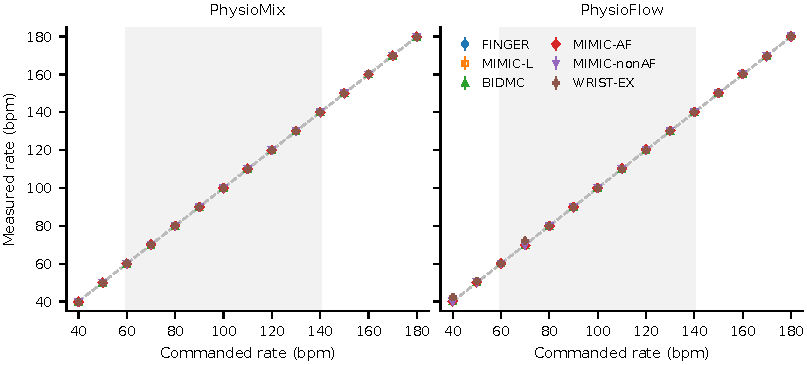
\includegraphics[width=\textwidth]{figures/fig5_rate_control.pdf}
\caption{Measured versus commanded rate for the deployed generators in the six recording contexts (median and interquartile range of eight strips per point, IBI CV command 0.02; laptop measurement). The shaded band marks 60--140\,bpm; the training labels cover 40--135\,bpm.}
\label{fig:rate}
\end{figure}

\subsection{Development under pre-specified rules}
\label{sec:res-development}

\begin{sidewaystable}
\centering
\caption{Decisions taken under rules fixed before training (or, for step A, before scoring). R9 and R10 are development rounds 9 and 10; R10-SB is the PhysioFlow-SB candidate judged by the round-10 rule. Gaps and margins in steps A--E are in percentage points of indistinguishability.}
\label{tab:decisions}
\footnotesize
\setlength{\tabcolsep}{4pt}
\begin{tabular}{>{\raggedright\arraybackslash}p{0.9cm}>{\raggedright\arraybackslash}p{3.0cm}>{\raggedright\arraybackslash}p{3.6cm}>{\raggedright\arraybackslash}p{8.0cm}>{\raggedright\arraybackslash}p{2.4cm}}
\toprule
Step & Candidate & Data used & Key comparison & Outcome \\
\midrule
\tablebody{tables/decisions.tex}
\bottomrule
\end{tabular}
\end{sidewaystable}

Table~\ref{tab:decisions} lists the decisions. Across rounds 3 to 7, PhysioMix improved from $\Sarm=0.596\pm0.026$ to $0.510\pm0.053$. Two kinds of change produced this progress. Generating a longer signal and cropping it (round 5) removed an artefact of circular filtering that the probe had learned to detect. The other changes concerned the critic: in round 5 every lazy R1 step hit the gradient-clipping limit, which weakened the penalty about tenfold; round 6 rescaled the limit, and round 7 reduced the R1 weight to 0.1. Round 9 added the motion term and the per-dataset distribution loss. It was accepted for its wrist gain (wrist $Q$ 0.527 versus 0.653), while its $\Sarm$ of 0.530 stayed within the allowed band. PhysioFlow reached a lower $\Sarm$ ($0.482\pm0.015$) and a lower probe AUC (0.703 versus 0.827), and its $\Sreal$ was within the non-inferiority margin, but its wrist $Q$ of 0.793 broke the wrist guard. It was therefore not deployed as the default and is offered in the application as a research mode. PhysioFlow-SB lowered $\Sarm$ further ($0.445\pm0.004$) and narrowed the wrist gap (0.597), but it again missed the guard, whose limit was 0.573.

\subsection{Realism on unseen subjects}
\label{sec:res-realism}

\begin{table}[tbp]
\centering
\caption{Realism on subjects never used for training. Each cell gives precision / recall / indistinguishable, all in \%, computed on up to 256 subject-balanced windows; $n$ is the number of unseen subjects among them (MIMIC-L has 316 unseen record groups, of which 191 were drawn). Real (other subjects) replaces the generator with real windows of training subjects. Intervals for the last value are in Table~\ref{tab:realism-ci}.}
\label{tab:realism}
\footnotesize
\resizebox{\textwidth}{!}{%
\begin{tabular}{lrccccc}
\toprule
Dataset & $n$ & PhysioMix & PhysioFlow & LSM-GAN & Gaussian & Real (other subjects) \\
\midrule
\tablebody{tables/realism.tex}
\bottomrule
\end{tabular}}
\end{table}

\begin{table}[tbp]
\centering
\caption{Indistinguishable (\%) on unseen subjects with 95\% subject-bootstrap intervals (Section~\ref{sec:stats}); point estimates as in Table~\ref{tab:realism}.}
\label{tab:realism-ci}
\footnotesize
\resizebox{\textwidth}{!}{%
\begin{tabular}{lrccccc}
\toprule
Dataset & $n$ & PhysioMix & PhysioFlow & LSM-GAN & Gaussian & Real (other subjects) \\
\midrule
\tablebody{tables/realism_ci.tex}
\bottomrule
\end{tabular}}
\end{table}

\begin{figure}[tbp]
\centering
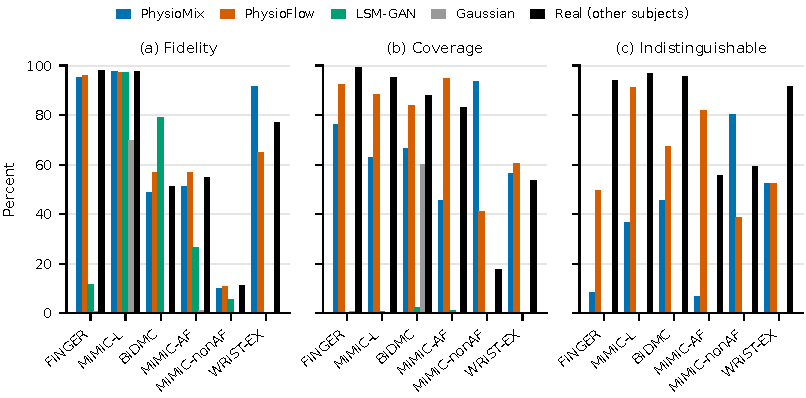
\includegraphics[width=\textwidth]{figures/fig6_realism.pdf}
\caption{Realism on subjects never used for training, by dataset and source (values of Table~\ref{tab:realism}; error bars, 95\% subject-bootstrap intervals).}
\label{fig:realism}
\end{figure}

Table~\ref{tab:realism} and Fig.~\ref{fig:realism} report realism per dataset. Both learned models placed most windows inside the real manifold on FINGER and MIMIC-L (precision 95--98\%), but they differed in recall and in how easily the probe found them. On FINGER, MIMIC-L, BIDMC and MIMIC-AF, PhysioFlow covered 84--95\% of the real windows and was 50--91\% indistinguishable; PhysioMix covered 46--76\% and was 7--45\% indistinguishable. The subject-bootstrap intervals (Table~\ref{tab:realism-ci}) separate the two models on FINGER (PhysioMix 9\%, 95\% interval 5--14\%, against PhysioFlow 50\%, 38--63\%), MIMIC-L (36\%, 29--43\%, against 91\%, 82--98\%) and MIMIC-AF (7\%, 3--12\%, against 82\%, 39--95\%), but overlap on BIDMC (45\%, 19--74\%, against 67\%, 41--91\%), which has 14 unseen subjects. Real windows of other subjects reached 94--97\% on FINGER, MIMIC-L and BIDMC, and PhysioFlow came closest to that level on MIMIC-L (91\% against 97\%). The order reversed on MIMIC-nonAF, where PhysioMix covered 94\% and was 80\% indistinguishable, but this dataset has two unseen subjects and real windows of other subjects reached only 59\%. On WRIST-EX the two models were equally detectable (52\%), and PhysioMix had the higher precision (92\% against 65\%). LSM-GAN produced plausible pulses on MIMIC-L and BIDMC (precision 97\% and 79\%) but covered at most 2\% of any dataset and was never indistinguishable, which is consistent with a collapse onto one pulse type; scored in its own 0.9--5\,Hz band on BIDMC, it reached 37\%. The Gaussian pulse was 0\% indistinguishable everywhere.

\subsection{Recording context and memorisation}
\label{sec:res-following}

\begin{sidewaystable}
\centering
\caption{Recording-context following and memorisation screening (Real, unseen: real windows of subjects never used for training). Balanced accuracy of a seven-class context classifier trained on real windows (chance 14\%), recognition of the wrist-exercise prompt, and the share of answers that follow the prompt when only the condition changes (swap). The last six columns give the median, over generated windows, of the maximum correlation with any training window of the same dataset.}
\label{tab:following}
\footnotesize
\setlength{\tabcolsep}{3pt}
\begin{tabular}{lrrrcccccc}
\toprule
 & \multicolumn{3}{c}{Context following (\%)} & \multicolumn{6}{c}{Median maximum correlation with training windows} \\
\cmidrule(lr){2-4}\cmidrule(lr){5-10}
Source & Balanced & Wrist-ex & Swap & FINGER & MIMIC-L & BIDMC & MIMIC-AF & MIMIC-nonAF & WRIST-EX \\
\midrule
\tablebody{tables/following.tex}
\bottomrule
\end{tabular}
\end{sidewaystable}

The context classifier recovered the prompted context for 54\% of PhysioMix windows and 68\% of PhysioFlow windows (balanced accuracy), against 51\% for real windows of unseen subjects (Table~\ref{tab:following}). When only the condition changed, 49\% (PhysioMix) and 71\% (PhysioFlow) of the answers followed it; LSM-GAN, which has no condition, stayed at chance. A score above the real level is not better. It suggests that PhysioFlow's windows are more typical of their context than real windows are, that is, less diverse. The wrist-exercise prompt was recognised in 77\% (PhysioMix) and 94\% (PhysioFlow) of cases, against 86\% for real wrist windows. The memorisation screen found no PhysioMix window with a correlation above 0.99 to a training window. For PhysioFlow, 0.8\% of BIDMC windows and 1.6\% of MIMIC-nonAF windows exceeded 0.99, which points to partial memorisation in the two smallest datasets. The median maximum correlations of both models were within 0.08 of those of real unseen windows, except for PhysioFlow on WRIST-EX (0.46 against 0.28).

\subsection{Beat detectors on generated strips}
\label{sec:res-detectors}

\begin{table}[tbp]
\centering
\caption{Share of windows (\%) whose rate a published beat detector estimated within 5\,bpm of the reference, with 95\% subject-bootstrap intervals. Real: recorded windows against ECG or Polar H10; generated strips against the rate of their scaffold, prompted with the reference rate of the paired real window and an IBI CV of 0.05. The context column gives subjects / windows. The last row averages, over the 12 context--detector cells, the absolute difference from the real value.}
\label{tab:detectors}
\footnotesize
\setlength{\tabcolsep}{4pt}
\begin{tabular}{llcccc}
\toprule
Context & Detector & Real & PhysioMix & PhysioFlow & Gaussian \\
\midrule
\tablebody{tables/detectors.tex}
\bottomrule
\end{tabular}
\end{table}

Table~\ref{tab:detectors} compares the detectors on real and generated data. Where the real recordings were clean, the generated strips matched them: on CapnoBase every detector estimated the rate within 5\,bpm on at least 99.6\% of real and generated windows, and on FINGER on 96\% of real windows (95\% interval 91--100\%) against 99--100\% of generated ones. Where the real recordings were hard, the strips did not follow. On WRIST-EX the detectors succeeded on only 19--26\% of the real windows, whose PPG is dominated by motion, but on 88--100\% of PhysioMix and PhysioFlow strips; on GalaxyPPG the figures were 75--77\% against 88--100\%. Averaged over the 12 context--detector cells, the generated strips were easier than the real data by 25.5 (PhysioMix) and 24.1 (PhysioFlow) percentage points, about as much as the Gaussian pulse (26.0). One failure appeared only in generated data: MSPTDfast succeeded on 88\% of the PhysioFlow strips prompted as wrist exercise, against 97--100\% for the other two detectors on the same strips, whereas on real wrist windows the three detectors differed by at most 7 points. No detector failed to find at least three beats in any window.

\subsection{Everyday wrist PPG and the independent judge}
\label{sec:res-wrist}

\begin{sidewaystable}
\centering
\caption{Everyday wrist PPG (GalaxyPPG, Empatica E4). (a) Fresh test of models trained without these data, over three halvings of all 24 participants. (b) Models retrained with GalaxyPPG, scored on the 12 participants held out from training; each row also gives the deployed PhysioMix and real windows of other participants from the same run. Indistinguishable is mean $\pm$ standard deviation across halvings (step E: mean over three seeds of the per-seed values). Rate error is the median absolute error against the prompted Polar rate.}
\label{tab:wrist}
\footnotesize
\textbf{(a)}\par\smallskip
\begin{tabular}{lrrrrrr}
\toprule
Source & Indist.\ (\%) & Precision (\%) & Recall (\%) & $Q$ & Rate error (bpm) & Within 5\,bpm (\%) \\
\midrule
\tablebody{tables/wrist_fresh.tex}
\bottomrule
\end{tabular}

\bigskip
\textbf{(b)}\par\smallskip
\setlength{\tabcolsep}{4pt}
\begin{tabular}{llrrrrrrr}
\toprule
 & & \multicolumn{3}{c}{Indistinguishable (\%)} & \multicolumn{2}{c}{$Q$} & & \\
\cmidrule(lr){3-5}\cmidrule(lr){6-7}
Step & Model & Model & PhysioMix & Real & Model & PhysioMix & Rate error (bpm) & Within 5\,bpm (\%) \\
\midrule
\tablebody{tables/wrist_retrain.tex}
\bottomrule
\end{tabular}
\end{sidewaystable}

\begin{figure}[tbp]
\centering
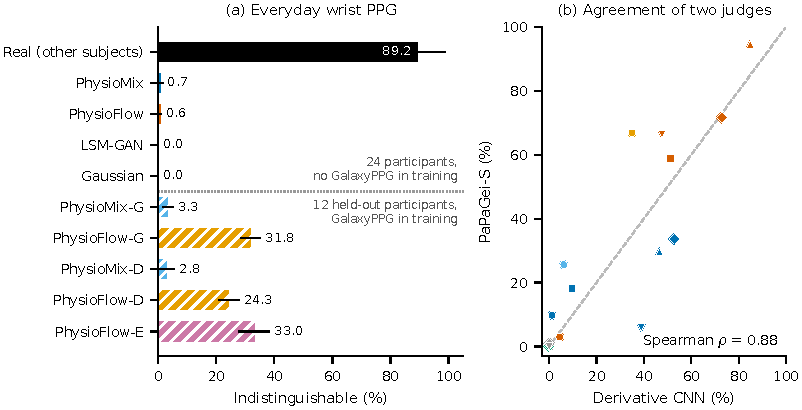
\includegraphics[width=\textwidth]{figures/fig7_wrist_judges.pdf}
\caption{(a) Indistinguishability on everyday wrist PPG. Upper block: fresh test of models trained without GalaxyPPG (24 participants). Lower block: models retrained with GalaxyPPG, scored on 12 held-out participants (hatched). Error bars: standard deviation across halvings. (b) Indistinguishability according to the derivative probe and to the frozen PaPaGei-S foundation model for 22 generator--dataset pairs (real data excluded). Colours identify the generator as in (a); markers identify the dataset: circle, GalaxyPPG; square, FINGER; upward triangle, MIMIC-L; diamond, BIDMC; downward triangle, WRIST-EX.}
\label{fig:wrist}
\end{figure}

Neither deployed model transferred to everyday wrist PPG (Table~\ref{tab:wrist}a). Over three halvings of the 24 GalaxyPPG participants, real windows of other participants were 89\% indistinguishable, PhysioMix 0.7\% and PhysioFlow 0.6\%; LSM-GAN and the Gaussian pulse were never indistinguishable. PhysioMix kept its rate accuracy (median error 1.5\,bpm) and had the best distribution score $Q$ among the generators (0.84). PhysioFlow did not meet the rule of step A, and PhysioMix remained the default.

Training on everyday wrist data changed the picture for the flow model only (Table~\ref{tab:wrist}b and Fig.~\ref{fig:wrist}a). With 12 GalaxyPPG participants in the wrist dataset (step B), PhysioFlow-G reached 31.8\% on the 12 held-out participants, against 0.7\% for the deployed PhysioMix and 3.2\% for the deployed PhysioFlow in the same run, but its wrist-exercise $Q$ on the original validation rose to 0.950 and breached the regression guard. Giving everyday wrist PPG its own dataset code (step D) removed this regression (0.574) and gave 24.3\% on the held-out participants. On the four validation participants, however, the gain over PhysioMix (28.8 points) fell short of the rule's margin of 32.8 points, twice the largest standard deviation across halvings. Step E used six validation participants and three seeds. The seeds agreed closely ($25.6\pm1.2\%$), but the standard deviation across halvings was 16.3 points, so the margin rose to 32.5 points and the gain of 25.6 points again fell short. The seed-mean wrist-exercise $Q$ on the original validation was 0.585, just inside its limit of 0.587 (one seed alone reached 0.684). On the held-out participants PhysioFlow-E reached 33.0\% (seed range 31.9--34.4\%) with a median rate error of 1.2\,bpm. PhysioMix retrained on the same data improved little (2.8--3.3\%).

PaPaGei-S ordered the generators much like our probe (Fig.~\ref{fig:wrist}b): over 22 generator--dataset pairs the Spearman correlation between the two indistinguishability scores was 0.88, and within datasets it ranged from 0.80 to 1.00. The foundation model was more lenient overall. On GalaxyPPG it rated PhysioMix 9.7\% and PhysioFlow-G 66.9\% indistinguishable, against 1.1\% and 35.0\% for the probe in the same run; it also placed the deployed PhysioMix above the deployed PhysioFlow (9.7\% against 2.9\%), the reverse of the probe (1.1\% against 4.5\%). The band-limited probes located what gives the deployed PhysioMix away on GalaxyPPG: it was 56\%, 80\% and 52\% indistinguishable in the 0.5--1.5, 1.5--3 and 3--5\,Hz bands, but 1\% in the 5--8\,Hz band, where real windows of other participants reached 89\%. The deployed PhysioFlow was given away in the same band (17\%).

\subsection{Computational footprint}
\label{sec:res-footprint}

On one laptop core, PhysioMix generated a 30\,s strip in 5.2\,ms, PhysioFlow in 716\,ms and LSM-GAN in 2.9\,ms (Table~\ref{tab:generators}). PhysioFlow is therefore about 140 times slower than PhysioMix and has 43 times more parameters. In the simulator it runs in the worker process and does not block the converter thread; its latency on the Raspberry Pi has not been measured.

%% ================================================================================================
\section{Discussion}
\label{sec:discussion}

\subsection{Separating rhythm from waveform}

Constructing the beat sequence and learning only the waveform around it gave a degree of rate control that the training data alone could not provide. The training labels cover 40--135\,bpm, yet both models met the command with mean errors below 1\,bpm up to 180\,bpm, because the scaffold sets the beat times and the learned part cannot move them. In PhysioMix the residual is bounded for this reason; in PhysioFlow the network is conditioned on the scaffold and was never asked to infer the rhythm when the scaffold was present. The same design limits what the models can learn about rhythm. The inter-beat intervals are log-normal and independent, so sequential patterns such as those of atrial fibrillation or ectopic beats are not reproduced and would need a rhythm model of their own \cite{solosenko2017af}. PhysioFlow nevertheless covered 95\% of the MIMIC-AF windows, which suggests that it learned the morphological changes that accompany an irregular rhythm even though the interval process was imposed.

\subsection{GAN or rectified flow}

On the finger and intensive-care datasets, rectified flow produced waveforms that the probe and the foundation model both found harder to separate from real ones, with higher recall and closer context following. The development history explains part of the difference. Two of the GAN rounds were spent on the stability of adversarial training (Section~\ref{sec:res-development}), whereas the flow model has a regression loss and no adversary, and its improvements came from the data path (when to supply the scaffold) and from the distribution of training times. The probe AUC tells the same story: 0.70 for PhysioFlow against 0.83 for PhysioMix on validation, although the GAN's critic was itself shown first and second differences. The price is compute. PhysioFlow needs 31 network evaluations per strip and about 140 times the CPU time of PhysioMix. For a simulator that generates 30\,s strips ahead of playback, this is acceptable on a laptop; on the Raspberry Pi it remains to be measured. The flow model is also less diverse: it followed contexts more consistently than real data do, and it showed signs of memorisation in the two smallest datasets. Both observations argue for more training subjects rather than for a larger network.

\subsection{What the beat detectors show}

The detector test separates two properties that the realism metrics mix. The learned strips look like real PPG to a probe and to a foundation model, yet they were as easy for beat detectors as the Gaussian pulse. The generators were prompted with a clean sinus rhythm and learned the pulse morphology of each context, but the difficulty of wrist PPG comes from motion and sensor artefacts that are not locked to the beat, and neither PhysioMix's periodic motion term nor PhysioFlow's wrist texture reproduced it. Part of the gap lies in the reference: a real window can disagree with its ECG or Polar rate even when the detector finds every pulse, whereas the rate of a generated strip is exact by construction, so the gap may overstate the difference in difficulty. The near-ceiling scores on CapnoBase and FINGER show that this effect is small on clean recordings, which suggests that most of the wrist gap reflects artefacts the generators lack. For users the consequence is direct: a detector that passes on these strips can still fail on wrist recordings, and the strips test rate and rhythm logic under controlled conditions rather than predict field performance. The realism metrics alone would not have shown this, which argues for an algorithm-level test in the evaluation of any PPG generator.

\subsection{Everyday wrist PPG and small validation sets}

Both deployed models failed on GalaxyPPG, and the band-limited probes show why: they reproduced the pulse bands but not the 5--8\,Hz texture of the E4 signal. Realism on one wrist dataset recorded with a research device during exercise did not carry over to a consumer device in daily life. Motion and sensor texture are device-specific, and a generator that targets wearables needs data from the class of device being tested. Training on the new device's data helped the flow model considerably, from 3.2\% for the deployed PhysioFlow to 24--33\% for the retrained flow models on the same held-out participants, and once these data had their own dataset code, the original validation stayed within the regression guards. Part of this gain may come from the stop-band loss of the PhysioFlow-SB recipe used for retraining rather than from the new data; we did not retrain the deployed recipe to separate the two.

The pre-specified rules did not let this result change the deployed model, and the reason deserves attention. The margin required a gain of twice the largest standard deviation of the scores across halvings, that is, a gain larger than most of the spread of single halvings, rather than a test of whether the mean gain differs from zero. With four or six validation participants, that spread (16 points in step E) was dominated by which participants served as the real reference: real windows of other participants themselves scored between 23\% and 100\% across the five halvings of step E. The candidate nevertheless exceeded the deployed PhysioMix in all 15 seed--halving pairs. A rule based on the paired differences, such as a one-sided paired test across halvings, would have had more power. We did not change the rule after seeing the scores, and such a rule would have to be tested on participants not yet used. In this case the rules probably cost us a better model for everyday wrist data. In others, such as round 10, they prevented a switch that the pooled score favoured but that would have undone the wrist improvement of round 9. We see this as the intended behaviour of fixing the analysis in advance \cite{nosek2018prereg}: with validation data reused over many rounds, a decision taken after seeing the scores would be hard to defend \cite{varoquaux2022failures}.

\subsection{Directions for the generators}

The results point to four directions. First, texture and motion: the 5--8\,Hz band and the motion that defeats detectors on wrist data are what the generators miss. A generator could take an accelerometer trace or a measured artefact as an additional input, so that motion is imposed like the rhythm rather than learned as a free periodic term; this keeps the test signal controllable and makes the difficulty of a strip a parameter rather than an accident. Second, sampling cost: PhysioFlow needs 31 network evaluations per strip. Reflow of the rectified flow \cite{liu2023rectified} or distillation into a consistency model \cite{song2023consistency} could reduce this to one or a few evaluations, which matters on the Raspberry Pi. Third, architecture and baselines: transformer diffusion models with an interpretable trend--season decomposition \cite{yuan2024diffusionts} and unified cardiovascular diffusion transformers \cite{chen2026unicardio} are natural external baselines, provided they are given the same constructed rhythm so that rate control is not lost. Fourth, physics: hybrid models that couple a light-transport or haemodynamic simulator to a learned correction \cite{behrmann2025hybrid,charlton2019pwdb} could provide paired infrared and red channels with a physical meaning, which our normalised single-channel view cannot. In each case the evaluation of this paper, including the detector test, would apply unchanged.

\subsection{What the generators can and cannot be used for}

The learned modes suit tests of beat detection, pulse-rate estimation and rhythm classification on waveforms whose rate and irregularity are known exactly, in a chosen recording context, with the caveat of Section~\ref{sec:res-detectors} that their strips are easier than real recordings. Robustness tests of denoising algorithms \cite{bradley2024envelope,jain2024ssl} or of sensors under vibration \cite{benkert2026vibration} would also benefit from strips whose ground-truth rhythm is known, once motion can be imposed. The learned modes do not suit SpO$_2$ testing. Each strip is a single normalised shape mapped to both channels with a fixed nominal ratio (Eq.~\ref{eq:mapping}), and the simulator's LEDs (625 and 875\,nm) differ from the 660 and 940\,nm pair that is common in pulse oximetry. The data view also removes the respiratory baseline, which the parametric mode still provides. Like other functional testers, the simulator does not establish SpO$_2$ accuracy \cite{iso80601}.

\subsection{Limitations}

All metrics are defined on a normalised 0.5--8\,Hz view without absolute amplitude or paired infrared and red channels; the FINGER dataset contains a red channel, which we stored but did not use. Several unseen cohorts are small (four subjects in MIMIC-AF and WRIST-EX, two in MIMIC-nonAF), so per-dataset estimates there are uncertain, as the intervals of Table~\ref{tab:realism-ci} show, and MIMIC-L subjects are record groups rather than verified patients. Validation data were reused over many development rounds, and the GalaxyPPG held-out participants had entered two earlier decisions. The decision rules were committed to our own repository, not registered with a third party. The detector test used three detectors from one library at the 40\,Hz rate of the data view and rate-level agreement only; beat-level timing errors were not assessed. The generators were timed on a laptop only, and the optical path of the simulator for which they were built has not been validated (\ref{app:hardware}). The labels are engineering labels, and nothing in this work is a clinical validation. The study comes from one laboratory.

%% ================================================================================================
\section{Conclusions}
\label{sec:conclusions}

We built two PPG generators that construct the beat sequence and learn the waveform around it. This made rate control exact for both a GAN and a rectified-flow model, and the flow model was markedly harder to tell apart from real PPG on finger and intensive-care data. Published beat detectors, however, found the generated strips about as easy as a Gaussian pulse and much easier than real wrist recordings, so a better realism score did not bring a more realistic difficulty. Neither model transferred to everyday wrist PPG from a new device without that device's data. With those data the flow model improved substantially, but not by the margin we had fixed in advance, and the pre-specified rules kept the deployed model unchanged. The next steps are to impose motion and sensor texture as controllable inputs, to reduce the number of flow steps, to learn paired infrared and red channels, to test a paired decision rule on participants not used so far, and to validate the optical path of the simulator.

%% ================================================================================================
\appendix
\section{Simulator hardware and real-time output}
\label{app:hardware}

\begin{figure}[tbp]
\centering
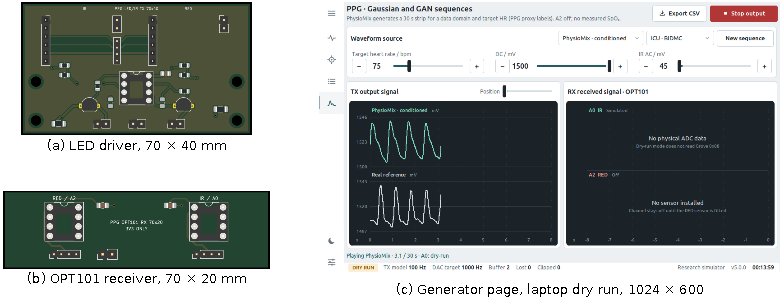
\includegraphics[width=\textwidth]{figures/fig2_hardware_ui.pdf}
\caption{(a, b) KiCad renders of the LED driver and OPT101 receiver boards, shown with empty sockets. (c) Generator page of the application in dry-run mode on a laptop at 1024\,$\times$\,600: a PhysioMix strip prompted for BIDMC at 75\,bpm (top trace) above a real training strip of the same dataset; the receiver card on the right reports that no ADC data exist instead of drawing a substitute.}
\label{fig:hardware}
\end{figure}

\paragraph{Hardware} A Raspberry Pi 4 Model B shares one I$^2$C bus between the two MCP4725 converters at addresses 0x60 (infrared command) and 0x61 (red command) and the analogue-to-digital converter of a Grove Base HAT, an MM32 microcontroller at address 0x08 that digitises 0--3.3\,V with 12 bits. The converters are supplied from the 3.3\,V rail, measured at 3.28\,V on our unit, so one code step corresponds to 0.80\,mV. Each converter output drives one LED through a voltage-controlled current sink (Fig.~\ref{fig:hardware}a). A 10\,k$\Omega$/10\,k$\Omega$ divider halves the command, and one half of an LM358 operational amplifier drives a 2N4401 transistor so that the voltage across the emitter resistor $R_s=100\,\Omega$ follows the divided command. The nominal emitter current is therefore
\begin{equation}
I_E \approx \frac{\vdac}{2R_s},
\label{eq:driver}
\end{equation}
about 16.4\,mA at full scale; the LED current is smaller by the base current. The LEDs are 3\,mm parts with a dominant wavelength of 620--625\,nm (red) and a peak wavelength of 875\,nm (infrared). Their anodes connect to the 5\,V rail, which supplies only the amplifier and the LEDs. Starting, stopping and closing the application park both converters at code 0, which turns the LEDs off. Light reaches one of two interchangeable receiver boards. The default board carries two OPT101 photodiode amplifiers \cite{opt101ds} with their internal 1\,M$\Omega$ feedback resistor and a 1\,k$\Omega$/1\,$\mu$F output filter (nominal cut-off 159\,Hz) ahead of the HAT inputs A0 (infrared) and A2 (red) (Fig.~\ref{fig:hardware}b). The alternative board uses BPW34 photodiodes with OPA333 transimpedance amplifiers (1\,M$\Omega$ in parallel with 22\,pF); integrated front-ends with ambient-light cancellation \cite{lin2019afe} would be the natural next step. A printed dark chamber separates the red and infrared lanes, holds the LEDs on sliding carriers and accepts apertures of 2, 5 and 16\,mm or a blank. The boards were designed in KiCad and pass its electrical-rule and design-rule checks. Their electrical and optical behaviour has not been measured; the bench capture below used an earlier assembly with an OPT101 module on A0 only.

\paragraph{Software} The touch interface is built with CustomTkinter, offers English and Vietnamese, and adapts to displays from 1024\,$\times$\,600 pixels upwards (Fig.~\ref{fig:hardware}c). The signal-engine thread evaluates the parametric model at 100\,Hz, interpolates linearly to the converter rate (100, 200, 500 or 1000\,Hz), stores the samples in a bounded ring buffer and writes both converters once per tick, infrared first. Writes are paced against absolute deadlines: the writer sleeps only for the time left before the next deadline and yields without sleeping when it is late. A lock serialises all converter writes, because the driver library shares one transmit buffer between instances. A receiver thread samples A0 and A2 at 100\,Hz and reports explicit states (live, stale, disabled, dry run and full scale) instead of drawing values when a sensor is absent. A Bluetooth Low Energy GATT server lets an Android application set parameters and receive the waveform at 50\,Hz with a 5\,Hz status message. Recordings store the commanded samples at 100\,Hz with timestamps, and the configuration is written atomically.

\paragraph{Measurements} On the Raspberry Pi 4 (Cortex-A72, Python 3.12.3, PyTorch 2.5.1), the engine counted, during 30\,s playbacks of an LSM-GAN strip, the samples generated, the deadlines missed by the writer (overruns), the samples dropped because the buffer was full, the reads that found the buffer empty (underruns) and the converter write errors (Table~\ref{tab:pi}). In the first headless run at 1\,kHz, a fixed sleep after the two I$^2$C writes made the writer fall behind: it missed 713 deadlines and dropped 802 samples in 30\,s. Sleeping only until the next deadline removed both. With the interface, the Bluetooth server and the receiver running, 1\,kHz still dropped 1{,}169 samples; skipping redraws of hidden pages and limiting the generator plot to 10 frames per second reduced the loss to 729. At 500\,Hz the same configuration generated 15{,}000 samples with no overrun, no dropped sample and no write error. The five underruns were ticks at which the writer found the buffer momentarily empty; no generated sample was dropped. We therefore made 500\,Hz the default on the Pi. The receiver sampled A0 at 99.995--100.002\,Hz in all phases of the capture. These counters describe the software only; the analogue output was not measured with an oscilloscope.

The PyTorch 2.10.0 wheel for aarch64 stopped with an illegal-instruction signal on the Cortex-A72, at an atomic instruction of the ARMv8.1 Large System Extensions that this ARMv8.0 core does not implement. PyTorch 2.5.1 ran correctly. On the Pi, the LSM-GAN TorchScript produced the same strip as on the laptop to within $2.4\times10^{-8}$\,V after the voltage mapping, and a cold start (import, load and generation) took 5.1\,s. The deployed PhysioMix and PhysioFlow generators were not timed on the Pi.

The optical loopback did not reproduce the waveform. During a 30\,s playback with only the infrared receiver connected, A0 stayed at the level recorded with the LEDs off for the first 22.5\,s and then jumped to a plateau near 3{,}300 counts. Over lags of $\pm250$\,ms, the largest absolute correlation between the detrended commanded and received signals was 0.045. We have not yet isolated the cause, which could lie in LED and receiver alignment, ambient light, grounding, receiver saturation or the driver stage, so the optical path remains unvalidated.

\begin{table}[tbp]
\centering
\caption{Converter output during 30\,s playbacks on the Raspberry Pi 4. Counters come from the signal engine; the analogue output was not measured with an oscilloscope.}
\label{tab:pi}
\footnotesize
\resizebox{\textwidth}{!}{%
\begin{tabular}{lrrrrrr}
\toprule
Configuration & Rate (Hz) & Generated & Overruns & Dropped & Underruns & Write errors \\
\midrule
\tablebody{tables/pi_timing.tex}
\bottomrule
\end{tabular}}
\end{table}

%% ================================================================================================
\section*{CRediT authorship contribution statement}
%% TODO(authors): confirm or edit the roles. The README credits hardware design and embedded firmware
%% to HuyNN and software design and UI/UX to VyPT.
\textbf{[First author]:} Conceptualization, Methodology, Investigation, Software, Formal analysis, Writing -- original draft. \textbf{[Second author]:} Software, Visualization, Validation, Writing -- review \& editing.

\section*{Declaration of competing interest}
%% TODO(authors): confirm.
The authors declare that they have no known competing financial interests or personal relationships that could have appeared to influence the work reported in this paper.

\section*{Data availability}
All training and test datasets are public: FINGER \cite{li2026mendeley}, MIMIC PERform \cite{charlton2025mimicperform}, BIDMC \cite{pimentel2017rr}, wrist PPG during exercise \cite{jarchi2017wrist}, GalaxyPPG (\url{https://doi.org/10.5281/zenodo.14635823}) \cite{park2025galaxyppg} and CapnoBase \cite{karlen2013capnobase}. Source code, board designs, trained generators with their SHA-256 digests, the pre-specified decision rules, the JSON records of the evaluation runs and the scripts that produce every figure and table of this paper from those records are available at \url{https://github.com/nguyenhuy0426/PPG_simulator}. The prepared data pack (49\,MB) is not redistributed; the preparation code in the repository builds it from the public sources, and its SHA-256 digest is recorded so that a rebuilt pack can be checked.
%% TODO(authors): cite the release tag or archive DOI of the submitted version. The code and frozen rules
%% of steps B-E and of PhysioFlow-SB are on branch claude/model-benchmark-physioflow-wrist-e-stopfix;
%% until it is merged and pushed, this statement is not true for them.

\section*{Funding}
%% TODO(authors): add grant information or keep this sentence.
This research did not receive any specific grant from funding agencies in the public, commercial, or not-for-profit sectors.

\section*{Acknowledgements}
We thank the creators of the BIDMC, MIMIC PERform, wrist PPG during exercise, FINGER, GalaxyPPG and CapnoBase datasets for making their recordings public, and the authors of PaPaGei and NeuroKit2 for releasing their models and software. GPU time was provided by Kaggle.

\section*{Declaration of generative AI and AI-assisted technologies in the manuscript preparation process}
%% Elsevier journal policy (updated June 2026): this section goes immediately before the references and
%% names the tool, its purpose and the extent of the authors' oversight. TODO(authors): after your own
%% revision, state what you checked (text, numbers, figures). AI help with the software, the board designs
%% or the experiments is research use and belongs in the Methods, not here.
During the preparation of this work the authors used Claude (Anthropic) to draft and edit the manuscript text and to write the scripts that draw every figure with Matplotlib (Fig.~\ref{fig:hardware} arranges KiCad renders and an application screenshot), generate the tables from the evaluation records and run the analyses of Sections~\ref{sec:detector-protocol} and \ref{sec:stats}. After using this tool, the authors reviewed and edited the content as needed and take full responsibility for the content of the published article.

\bibliographystyle{elsarticle-num}
\bibliography{refs}

\end{document}
